\chapter{Methodology}

\section{Study Objective and Experimental Strategy}

The objective of this thesis is the approximation of basket option prices using a VQC and the comparison with classical ANNs (Culkin and Ferguson architectures).

In addition to the model comparison, it is investigated to what extent predictive performance depends on the underlying payoff structure. For this purpose, three different basket types are considered: \textit{Worst-of}, \textit{Best-of}, and \textit{Average}. These exhibit different functional properties and nonlinearities and therefore represent approximation tasks of varying complexity.

Due to the structurally different model architecture of a VQC, it is analyzed whether differences in generalization ability emerge under reduced training data availability compared to classical neural networks. 
This investigation is motivated by empirical studies suggesting that quantum neural networks may exhibit improved robustness when learning from scarce and noisy datasets compared to classical approaches \cite{stein2023benchmarking}.

Furthermore, it is examined to what extent the models differ in their robustness to noisy training data. For this purpose, controlled artificial noise is added to the training targets in order to analyze sensitivity to perturbed labels.

In addition to studying these two effects in isolation (limited data and increased noise), their combined influence is also analyzed to identify potential interaction effects between sample size and noise intensity.

Finally, in addition to a random train-test split, a temporally ordered split is considered. This serves to evaluate generalization performance under more realistic conditions, where only past information is used to predict future values.

\section{Data Generation}
\label{sec:mt-data-generation}

To investigate whether VQCs offer advantages in representing correlations between assets through entanglement, real market prices of basket options would ideally be required.
However, such consistent and freely available datasets exist only to a limited extent.

Therefore, historical time series of individual underlyings are used to generate the target values.
Based on the volatilities and correlation structures estimated from these data, synthetic basket option prices are generated using Monte Carlo simulation.

\subsection{Market Data and Parameter Estimation}
\label{sec:mt-market-data}

For the Monte Carlo simulation, the volatilities of the individual assets as well as their correlations are required. These parameters are estimated from historical market data.

The input data consist of daily closing prices (\textit{close prices}) of the respective underlyings. Based on these prices, logarithmic returns (log returns) are computed:
\begin{equation}
r_t = \ln\left(\frac{S_t}{S_{t-1}}\right),
\label{eq:log-returns}
\end{equation}
where $S_t$ denotes the closing price on trading day $t$.

From the log returns, rolling volatilities over a window of length $w$ are estimated and annualized:
\begin{equation}
\sigma_{\text{ann}, t}^{w}
=
\sigma_{t}^{w} \cdot \sqrt{D},
\end{equation}
where $D = 252$ denotes the assumed number of trading days per year.

The correlation between the underlyings is also determined empirically based on the log returns:
\begin{equation}
\rho_{ij}
=
\frac{
    \sum_{t=1}^{T}
    \left(r_{t}^{i} - \bar{r}^{i}\right)
    \left(r_{t}^{j} - \bar{r}^{j}\right)
}{
    \sqrt{
        \sum_{t=1}^{T} \left(r_{t}^{i} - \bar{r}^{i}\right)^{2}
    }
    \sqrt{
        \sum_{t=1}^{T} \left(r_{t}^{j} - \bar{r}^{j}\right)^{2}
    }
},
\label{eq:corr}
\end{equation}
where
\begin{equation}
\bar{r}^{i} = \frac{1}{T} \sum_{t=1}^{T} r_{t}^{i}
\end{equation}
denotes the mean return of the $i$-th asset.

To ensure that the correlation matrix is suitable for Cholesky decomposition, it is approximated by the nearest positive definite matrix (cf.~\cite{higham1988computing}).

\subsection{Monte Carlo Basket Pricing}
\label{sec:mt-monte-Carol}

To compute the basket option prices, the Monte Carlo procedure described in Section~\ref{sec:bg-monte-carlo} is used.

Since the volatilities are given in annualized form, the remaining time to maturity of the option is converted into years:
\begin{equation}
T_{\text{years}} = \frac{T}{D}.
\end{equation}

For each simulation path, standard normally distributed random vectors are generated, correlated via the Cholesky decomposition of the correlation matrix, and subsequently substituted into the pricing equation~\eqref{eq:bg-GBM}.

The risk-free interest rate is set to $r = 0$ in all experiments. As a result, discounting of the payoffs is omitted, and the average of the simulated payoffs directly serves as an estimator of the fair option price.

To avoid distortions due to different absolute initial price levels of the underlyings, valuation is performed on the basis of relative terminal prices rather than absolute prices.

For the $i$-th asset, the following is defined:
\begin{equation}
G_i = \frac{S_T^{i}}{S_0^{i}}.
\end{equation}

Thus, valuation depends exclusively on the relative performance of the underlyings.

The strike prices are also defined in relative terms.
For each market observation, a set of $M = 5$ strike values is generated
to represent different moneyness levels.

The relative strikes $m$ are drawn independently and uniformly
from a fixed interval
\[
m \sim \mathcal{U}(0.7, 1.3).
\]
This interval corresponds to the strike range used in
\cite{culkin2017machine}, defined relative to the spot price.

By using relative terminal prices, the valuation becomes invariant with respect to the absolute initial price levels of the underlyings. The payoff is multiplied by a fixed notional of $1$.

Based on the relative terminal prices $G_i$ and the relative strike $m$, the considered basket payoffs are given by

\begin{align}
\text{Worst-of:} \quad &
\max\!\left(\min_{i} G_i - m,\, 0\right), \\
\text{Best-of:} \quad &
\max\!\left(\max_{i} G_i - m,\, 0\right), \\
\text{Average:} \quad &
\max\!\left(\frac{1}{n}\sum_{i=1}^{n} G_i - m,\, 0\right).
\end{align}

The mean of these payoffs over all $n_{\text{paths}} = 1{,}000{,}000$ simulated paths serves as the Monte Carlo estimator of the option price.

% In addition to pure price estimation, further statistical quantities are recorded during the Monte Carlo simulation to analyze structural properties of the payoff functions. These include:

% \begin{itemize}
%     \item the dominating underlying per simulation path,
%     \item the frequency of dominating assets (\textit{counts}),
%     \item the conditional mean payoffs per asset (\textit{means}).
% \end{itemize}

\section{Model Specification}

\subsection{Culkin Architecture}
\label{sec:mt-culkin}

The first architecture is based on \cite{culkin2017machine} and combines fully connected layers with dropout regularization.
A total of four hidden layers with $u$ neurons each are used, where the activation functions vary across layers. Specifically, the sequence
\[
\text{LeakyReLU} \rightarrow \text{ELU} \rightarrow \text{ReLU} \rightarrow \text{ELU}
\]
is applied. After each hidden layer, dropout with rate $p$ is used.
The output layer consists of a single neuron with exponential activation, ensuring that the model prediction is strictly positive. The total number of trainable parameters is
\begin{equation}
\label{eq:params_culkin}
P_{\text{Culkin}}
=
(d+1)u
+ 3(u+1)u
+ (u+1).
\end{equation}

\subsection{Ferguson Architecture}
\label{sec:mt-ferguson}

The second architecture follows \cite{ferguson2018deeply}.
A fully connected feedforward network is employed, consisting of an input layer, six hidden layers with $u$ neurons each, and a linear output layer. The ReLU activation function is used in all hidden layers.
The output $\hat{y}$ represents the model prediction of the basket price.
The total number of parameters of this model is given by
\begin{equation}
\label{eq:params_ferguson}
P_{\text{Ferguson}}
=
(d+1)u
+ 5(u+1)u
+ (u+1),
\end{equation}
where the term $+1$ accounts for the bias in each layer.

\subsection{Variational Quantum Circuit}
\label{sec:mt-vqc-model}

As a quantum-based model, a VQC is employed, whose fundamental structure was introduced in Section~\ref{sec:bg-vqc}.
In the following, the specific architecture used in this thesis is described.

\subsubsection{Number of Qubits}

Each input feature $x_n$ is assigned exactly one qubit, such that the data are encoded in parallel. The number of qubits therefore equals the input dimension $d$:
\begin{equation}
n_{\text{qubits}} = d.
\end{equation}

\subsubsection{Data Encoding}

As described in Section~\ref{subsubsec:bg-vqc-architecture},
in principle any Pauli operator can be used as the Hamiltonian for data encoding.

In the present work, a rotation-based encoding using $R_X$ gates is employed. For each input component $x_n$, a rotation of the form
\[
R_X(p_l x_n)
\]
is applied in every layer $l$.

Two different scaling schemes are considered:

\paragraph{Unary Encoding.}
In unary encoding, no layer-specific prefactor is used, i.e.,
\[
p_l = 1 \quad \forall l.
\]
The input data are thus reuploaded identically in each layer.

\paragraph{Ternary Encoding.}
In ternary encoding, an exponentially increasing prefactor is chosen:
\[
p_l = 3^{\,l-1}.
\]

\subsubsection{Trainable Blocks}

Between the data encoding layers, trainable ansatz layers $W^{(l)}(\theta_l)$ are inserted. Each ansatz layer consists of $B$ train blocks $W^{(l)}_b(\theta_{l,b})$ with $b = 1, \dots, B$.

A single train block is structured as follows:

\begin{itemize}
    \item First, a general single-qubit rotation is applied to the first qubit.
    \item Subsequently, a linear CNOT ladder is implemented between neighboring qubits.
    \item After each CNOT gate, a general rotation operation is applied again to the respective target qubit.
\end{itemize}

The ladder structure has the advantage that, compared to fully connected entanglement patterns, the effective circuit depth remains lower. This helps to avoid excessive global randomization of the state space, which may reduce the emergence of highly concentrated gradient distributions. At the same time, the structured coupling of neighboring qubits enables the modeling of non-separable dependencies between the input variables.

The general rotation operation is defined as
\begin{equation}
\mathrm{Rot}(\theta^{(l)}_{b,j})
=
\mathrm{Rot}\!\left(
\theta^{(l,1)}_{b,j},
\theta^{(l,2)}_{b,j},
\theta^{(l,3)}_{b,j}
\right),
\end{equation}
where $j$ denotes the qubit index, $b$ the index of the train block, and $l$ the index of the Ansatz layer.
In the PennyLane implementation used here, the rotation consists of successive rotations around the $z$-, $y$-, and $z$-axes \cite{pennylane_rot}.

The structure of a ladder sub-block is illustrated in
Figure~\ref{fig:w-ladder-block}.

\begin{figure}[htbp]
\centering
\begin{quantikz}[row sep=0.1cm, column sep=0.15cm]
\lstick{$0$}
  & \gate{\mathrm{Rot}(\theta_{b,0})}
  & \ctrl{1} & \qw       & \qw       & \qw & \qw & \qw \\
\lstick{$1$}
  & \qw
  & \targ{}
  & \gate{\mathrm{Rot}(\theta_{b,1})}
  & \ctrl{1} & \qw & \qw & \qw \\
\lstick{$2$}
  & \qw
  & \qw
  & \qw
  & \targ{}
  & \gate{\mathrm{Rot}(\theta_{b,2})}
  & \ctrl{1} & \qw \\
\lstick{$3$}
  & \qw
  & \qw
  & \qw
  & \qw
  & \qw
  & \targ{}
  & \gate{\mathrm{Rot}(\theta_{b,3})}
\end{quantikz}
\caption{Train block $W^{(l)}_b(\theta_{l,b})$ for $d=4$ qubits.
After an initial rotation on the first qubit, a linear CNOT ladder is implemented between neighboring qubits. After each CNOT gate, a general rotation operation is applied to the corresponding target qubit.
The parameter $\theta_{b,j}$ denotes the full set of associated rotation parameters.}
\label{fig:w-ladder-block}
\end{figure}

\subsubsection{Overall Architecture}

The complete circuit consists of an initial Ansatz layer $W^{(0)}(\theta_0)$, followed by $L$ alternating sequences of data encoding and Ansatz layers $W^{(l)}(\theta_l)$, $l = 1, \dots, L$.

The overall structure is schematically illustrated in
Figure~\ref{fig:full-vqc}.

\begin{figure}[htbp]
\centering
\begin{quantikz}[row sep=0.25cm, column sep=0.30cm]
    \lstick{$\ket{0}$} & \gate[wires=4]{W^{(0)}} & \gate{R_X(x_0)} & \qw & \gate[wires=4]{W^{(1)}} & \gate{R_X(3 x_0)} & \qw & \gate[wires=4]{W^{(2)}} & \gate{R_X(9 x_0)} & \qw & \gate[wires=4]{W^{(3)}} & \qw & \qw \\
    \lstick{$\ket{0}$} & \qw & \gate{R_X(x_1)} & \qw & \qw & \gate{R_X(3 x_1)} & \qw & \qw & \gate{R_X(9 x_1)} & \qw & \qw & \qw & \qw \\
    \lstick{$\ket{0}$} & \qw & \gate{R_X(x_2)} & \qw & \qw & \gate{R_X(3 x_2)} & \qw & \qw & \gate{R_X(9 x_2)} & \qw & \qw & \qw & \qw \\
    \lstick{$\ket{0}$} & \qw & \gate{R_X(x_3)} & \qw & \qw & \gate{R_X(3 x_3)} & \qw & \qw & \gate{R_X(9 x_3)} & \qw & \qw & \qw & \meter{}
\end{quantikz}
\caption{Overall architecture of the VQC (example $d=4$, $L=3$):
Initial Ansatz layer $W^{(0)}(\theta_0)$, followed by alternating data-encoding layers $R_X(3^{l-1}x_n)$ and Ansatz layers $W^{(l)}(\theta_l)$. The measurement is performed on the last qubit.}
\label{fig:full-vqc}
\end{figure}

\subsubsection{Model Output}

The model prediction is defined as the expectation value of the
Pauli-$Z$ operator on the last qubit:
\begin{equation}
f_\theta(x)
=
\langle 0^{\otimes d} |
U^\dagger(x,\theta)\,
Z_{d-1}\,
U(x,\theta)
| 0^{\otimes d} \rangle.
\end{equation}

\subsubsection{Number of Parameters}

A single train block contains one general rotation per qubit with three free parameters. Thus, per train block,

\begin{equation}
P_{\text{block}} = 3d.
\end{equation}

Since each Ansatz layer consists of $B$ train blocks and a total of $L+1$ Ansatz layers are used, the total number of trainable parameters is

\begin{equation}
\label{eq:params_vqc}
P_{\text{VQC}} = 3d \cdot B \cdot (L+1).
\end{equation}

\subsubsection{Dynamical Lie Algebra and Effective Degrees of Freedom}

The expressive power of the model is additionally determined by the dimension
of the DLA $\mathfrak{g}$
(cf.\ Section~\ref{sec:bg-vqc-trainable-blocks}).
Since the employed ansatz contains general single-qubit rotations and
CNOT gates, it can in general generate the full
Lie algebra. For a system with $d$
qubits, this yields

\begin{equation}
\dim(\mathfrak{g}) = 4^d - 1 .
\end{equation}

Since the circuit consists of $L+1$ ansatz layers separated by
data-encoding operations, the following upper bound
for the number of effectively controllable Fourier coefficients is obtained

\begin{equation}
F_{\text{eff}} \le (L+1)(4^d - 1).
\end{equation}

\section{Frequency Analysis of the Target Functions}
\label{sec:mt-frequency-analysis}

As shown in Section~\ref{sec:bg-vqc-fourier}, the model function of a rotation-based VQC can be expressed as a finite Fourier series, where the representable frequency spectrum $\Omega$ depends on the encoding depth $L$.

To analyze the frequency components contained in the target functions, the adjoint NUFFT described in Section~\ref{sec:bg-nufft} is employed.
From the training data, approximate Fourier coefficients $\hat{c}_\omega$ are computed on a predefined frequency grid.

Since the input dimension satisfies $d > 2$, a direct visualization of the full multidimensional frequency spectrum is not feasible.
Therefore, two-dimensional projections are used for representation.

To this end, the amplitude spectrum
\[
|\hat{c}_\omega|
\]
is first summed over all frequency axes that are not displayed.
For two selected dimensions $p$ and $q$, the projected amplitude is given by

\begin{equation}
A_{p,q}(\omega_p, \omega_q)
=
\sum_{\omega_k,\, k \notin \{p,q\}}
|\hat{c}_\omega|.
\end{equation}

For improved comparability, the projected amplitude is subsequently normalized:

\begin{equation}
\widetilde{A}_{p,q}(\omega_p, \omega_q)
=
\frac{
A_{p,q}(\omega_p, \omega_q)
}{
\max_{\omega_p,\omega_q}
A_{p,q}(\omega_p, \omega_q)
}.
\end{equation}

\section{Training Procedure}
\label{sec:mt-training}

All models are trained by minimizing the MSE between the predicted basket option prices and those generated via Monte Carlo simulation.

The Adam optimizer with a learning rate of 0.001 is used, corresponding to a standard choice frequently adopted in the literature.
To ensure comparable training duration across different training dataset sizes, training is defined by a fixed number of optimization steps rather than a fixed number of epochs.

The batch size is chosen automatically depending on the number of available training samples and is set to $10\%$ of the training set size.
It is constrained to a minimum of $8$ and a maximum of $64$.
The effective number of epochs is implicitly determined by the chosen batch size and the predefined number of optimization steps.

\section{Evaluation Metrics}
\label{sec:mt-evaluation-metrics}

The predictive performance of the models is evaluated exclusively on the test data.

As the primary evaluation metric, the coefficient of determination
$R^2$ is used:
\begin{equation}
R^2
=
1 - \frac{\sum_{i=1}^{N_{\text{test}}}(y_i - \hat{y}_i)^2}
{\sum_{i=1}^{N_{\text{test}}}(y_i - \bar{y})^2},
\end{equation}
where $y_i$ denotes the simulated target values,
$\hat{y}_i$ the model predictions, and
$\bar{y}$ the mean of the target values
in the test dataset.

Since $R^2$ is bounded above by $1$ but has no fixed lower bound,
individual outliers may strongly affect the arithmetic mean.
For this reason, the median of the test $R^2$ values
across multiple random seeds is reported in the results.

\section{Experimental Setup}
\label{sec:mt-experimental-setup}

\subsection{Dataset}
\label{sec:mt-dataset}

For the experiments, the two underlyings
\texttt{IBM} and \texttt{NKE} are considered.
Daily closing prices from 01.01.2000 to 01.01.2025 are used,
obtained from \texttt{Yahoo Finance}.

The input data consist of the volatilities of both underlyings
as well as the relative strike.
The input vector is given by
\[
x = (\sigma_{\text{IBM}}, \sigma_{\text{NKE}}, m) \in \mathbb{R}^3.
\]

For each $x$, three target values are determined via Monte Carlo simulation:
a Worst-of, a Best-of, and an Average payoff.
The three resulting target quantities are not modeled jointly;
instead, a separate model is trained for each scenario,
using only a single target value $y = f(x)$.

\subsection{Data Split}
\label{sec:mt-data-split}

The available data are divided into training and test sets.
By default, a random train-test split is applied,
with $20\%$ of the observations assigned to the test set
and the remaining $80\%$ to the training set.

The split is performed in a group-wise manner by date,
since for each trading day $M = 5$ relative strikes are available.
This prevents identical volatility values with different strikes
from being distributed across training and test sets,
thereby avoiding data leakage.

The input features and target values are accordingly divided into
$X_{\text{train}}, X_{\text{test}}$
and
$Y_{\text{train}}, Y_{\text{test}}$.

\subsection{Computation of the Frequency Structure of the Target Functions}
\label{sec:mt-computed-spectrum}

To analyze the frequencies representable by the VQC,
the spectral amplitudes are computed on a frequency grid
with $N = 31$, as described in Section~\ref{sec:mt-frequency-analysis}.

\begin{figure}[htbp]
\centering
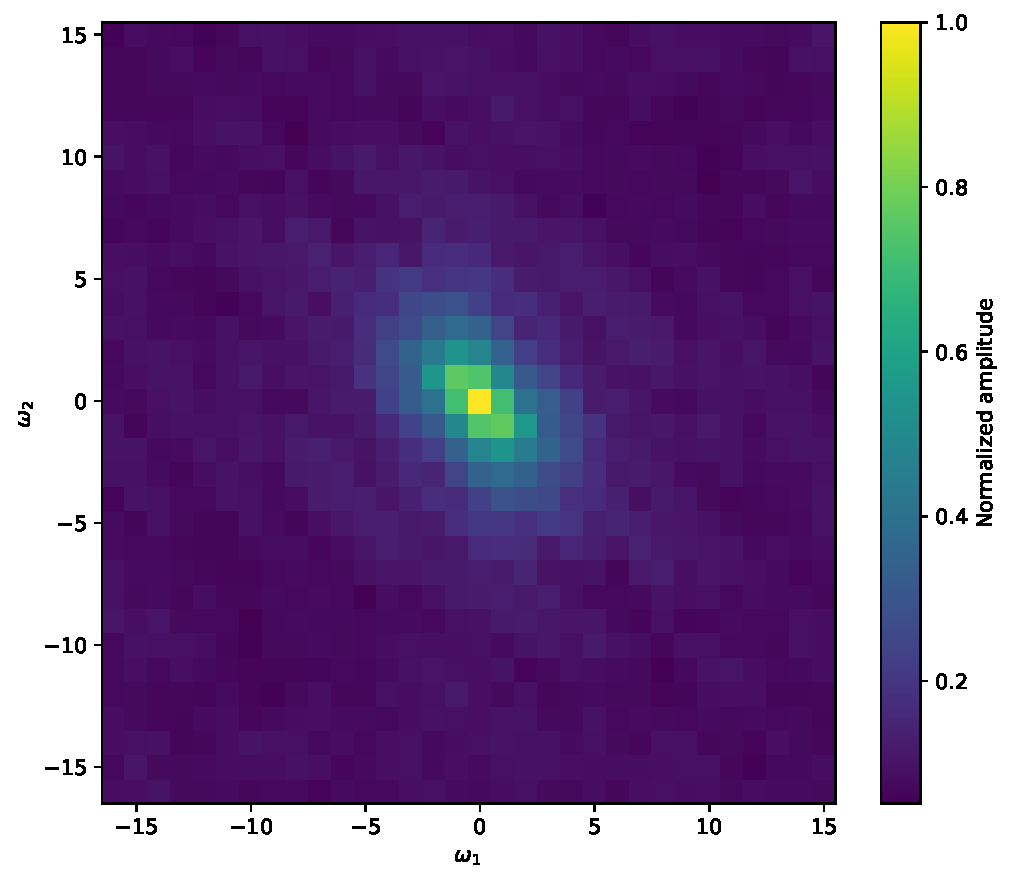
\includegraphics[width=0.6\linewidth]{pictures/plot_spectrum.pdf}
\caption{Two-dimensional projection of the normalized amplitude spectrum of the training data over the two volatility dimensions. 
The projection is obtained by summing over the strike dimension.}
\label{fig:spectrum_projection}
\end{figure}

Figure~\ref{fig:spectrum_projection} shows the projected
frequency structure of the target functions.
The multidimensional spectrum is summed over the strike dimension
and subsequently normalized, such that relative intensities
become visible.

The amplitudes are clearly concentrated in the low-frequency range.
Most of the spectral mass lies within
$|\omega_n| \leq 1$, while the intensity decreases steadily
with increasing frequency.
Frequency components with $|\omega_n| \geq 5$ are only weakly pronounced.

This structure indicates that the target functions
can predominantly be described by low frequencies.
Since the representable spectrum of a rotation-based VQC
grows with encoding depth,
a small depth is likely sufficient to capture the dominant components.
Increasing the encoding depth to cover frequencies up to approximately
$|\omega_n| \leq 4\text{--}5$ per input dimension
may further improve the approximation,
whereas beyond this range only limited additional
performance gains are to be expected.



\subsection{Model Configurations}
\label{sec:mt-model-config}

\subsubsection{Variational Quantum Circuits}

For the VQCs, encoding depths
$L \in \{1,3,4,5\}$ are considered for unary encoding,
while for ternary encoding
the encoding depths $L \in \{2,3\}$ are used.
This allows the frequency spectra computed in
Section~\ref{sec:mt-computed-spectrum} to be represented.

The size of the entire frequency spectrum for unary encoding is

\[
|\Omega| = (2L+1)^d .
\]

(cf.~Section~\ref{sec:bg-vqc-fourier}).
For ternary encoding, Equation~\ref{eq:Omega_n} yields

\[
|\Omega| = 3^{Ld}
\]

(cf.~Section~\ref{sec:bg-vqc-frequency-scaling}).

For $d=3$ input dimensions, for example,
for $L=2$ (ternary encoding) with $p_1=1$ and $p_2=3$ per dimension we obtain

\[
\Omega_n =
\{-4,-3,-2,-1,0,1,2,3,4\},
\]

such that $|\Omega_n| = 9$ and

\[
|\Omega| = |\Omega_n|^d = 9^3 = 729.
\]

For the considered encoding depths, this results in:

\begin{table}[htbp]
\centering
\begin{tabular}{c c c c}
\hline
Encoding & $L$ & Frequency range $|\omega_n|$ & $|\Omega|$ \\
\hline
Unary   & 1 & $\le 1$  & 27   \\
Unary   & 3 & $\le 3$  & 343  \\
Unary   & 4 & $\le 4$  & 729  \\
Unary   & 5 & $\le 5$  & 1331 \\
\hline
Ternary & 2 & $\le 4$  & 729  \\
Ternary & 3 & $\le 13$ & 19683 \\
\hline
\end{tabular}
\caption{Size of the achievable frequency spectrum for the considered
encoding depths with $d=3$ input dimensions.}
\label{tab:frequency-spectra}
\end{table}

To provide a sufficient number of trainable parameters for controlling
the representable Fourier coefficients,
the number of ladder sub-blocks $B$ is chosen depending on $L$ as

\[
(L,B) \in \{(1,10), (3,10), (4,17), (5,25)\}
\]

for unary encoding and

\[
(L,B) \in \{(2,20), (3,30)\}
\]

for ternary encoding.

\subsubsection{Classical Neural Networks}

For the Culkin architecture, four hidden layers
with $u=100$ neurons each and a dropout rate
of $p=0.25$ are used, corresponding to the
original configuration in the reference paper.

For the Ferguson architecture, several
variants are considered:
\begin{itemize}
    \item a configuration with $u=100$ neurons
    per hidden layer without dropout,
    analogous to the original work,
    \item as well as reduced variants with
    $u \in \{5,9,14\}$ neurons per hidden layer,
    whose number of parameters is adjusted
    to match those of the QML models.
\end{itemize}

\subsubsection{Comparison of Model Complexity}

To ensure a fair comparison between
classical neural networks and the VQC,
models with a comparable number of trainable
parameters are explicitly contrasted.
In this way, differences in predictive performance
can be attributed less to differing model capacity
and more to structural properties of the architectures.

The total number of trainable parameters
of the considered model configurations
is shown in Table~\ref{tab:model-parameters}.

\begin{table}[htbp]
\centering
\begin{tabular}{l c c}
\hline
Model & Parameters & $F_{\text{eff}}$ \\
\hline
QML (Unary, $L=1$, $B=10$) & 180 & $126$ \\
QML (Unary, $L=3$, $B=10$) & 360 & $252$ \\
QML (Unary, $L=4$, $B=17$) & 765 & $315$ \\
QML (Unary, $L=5$, $B=25$) & 1350 & $378$ \\
QML (Ternary, $L=2$, $B=20$) & 540 & $189$ \\
QML (Ternary, $L=3$, $B=30$) & 1080 & $252$ \\
\hline
Ferguson ($u = 5$) & 176 & -- \\
Ferguson ($u = 9$) & 496 & -- \\
Ferguson ($u = 14$) & 1121 & -- \\
Ferguson ($u = 100$) & 51001 & -- \\
Culkin ($u = 100$, $drop=0.25$) & 30801 & -- \\
\hline
\end{tabular}
\caption{Number of trainable parameters and maximum number of effectively controllable Fourier coefficients of the considered models.}
\label{tab:model-parameters}
\end{table}

\subsection{Baseline Scenario}
\label{sec:mt-baseline}

As a reference point for the subsequent experiments,
a baseline scenario is first considered.

In this setting, the full training dataset resulting
from the random train-test split
(cf.~Section~\ref{sec:mt-data-split})
is used. No artificial reduction
of the training data is applied.

\subsection{Reduced Training Data}
\label{sec:mt-low-data}

To investigate the generalization capability
of the models under limited data availability,
the size of the training set is reduced.

For this purpose, a random subset of the original
training dataset with
$N_{\text{train}} \in \{\;25,\;50,\;100,\;250,\;500,\;1000\}$
observations is drawn.
The test dataset remains unchanged,
ensuring comparability of the results.

\subsection{Noise Robustness}
\label{sec:mt-noise}

To examine robustness to noisy training data,
artificial noise is added to the training targets.

The noise term follows the approach proposed in
\cite{mitarai2018quantum}.
Gaussian noise of the form

\begin{equation}
    \varepsilon = \alpha \cdot \mathcal{N}(0,1)
\end{equation}

is used, where $\alpha$ denotes a scaling parameter
controlling the noise intensity.

To scale the noise relative to the magnitude
of the target values, the noise term is applied
multiplicatively to the training targets:

\begin{equation}
    \widetilde{Y}_{\text{train}} = Y_{\text{train}} \,(1 + \varepsilon).
\end{equation}

The test targets $Y_{\text{test}}$ remain unchanged
in all experiments.

The following values are considered:

\[
\alpha \in \{0, 0.05, 0.1, 0.25, 0.5\}.
\]

\subsection{Reproducibility and Random Initialization}
\label{sec:mt-seeds}

To assess the stability of the results with respect
to random influences, all experiments are repeated
over 30 different random initializations (seeds).

The respective seed affects

\begin{itemize}
    \item the random train-test split,
    \item the random selection of reduced training subsets,
    \item the realization of artificial noise,
    \item as well as the initialization of the model parameters.
\end{itemize}

The results are aggregated across all seeds.
The quantum models are fully reproducible given a fixed seed,
whereas classical neural networks may exhibit minor deviations
due to non-deterministic hardware operations and GPU-based
parallel reductions \cite{tensorflow_determinism}.

\section{Implementation Details}
\label{sec:mt-implementation-details}

The quantum machine learning models are implemented using the
\texttt{PennyLane} library \cite{bergholm2018pennylane}.
For efficient circuit evaluation, the JAX interface \cite{bradbury2018jax}
is employed.
The classical neural networks are implemented using
\texttt{TensorFlow/Keras} \cite{abadi2015tensorflow}.
For all models, fixed random seeds are used
to ensure training runs that are as reproducible as possible.